\chapter{Heartbeat}
\label{chap:heartbeat}

In this chapter, we discuss what information a heartbeat contains and how it is processed by the masterserver.

\begin{figure}[ht]
\centering
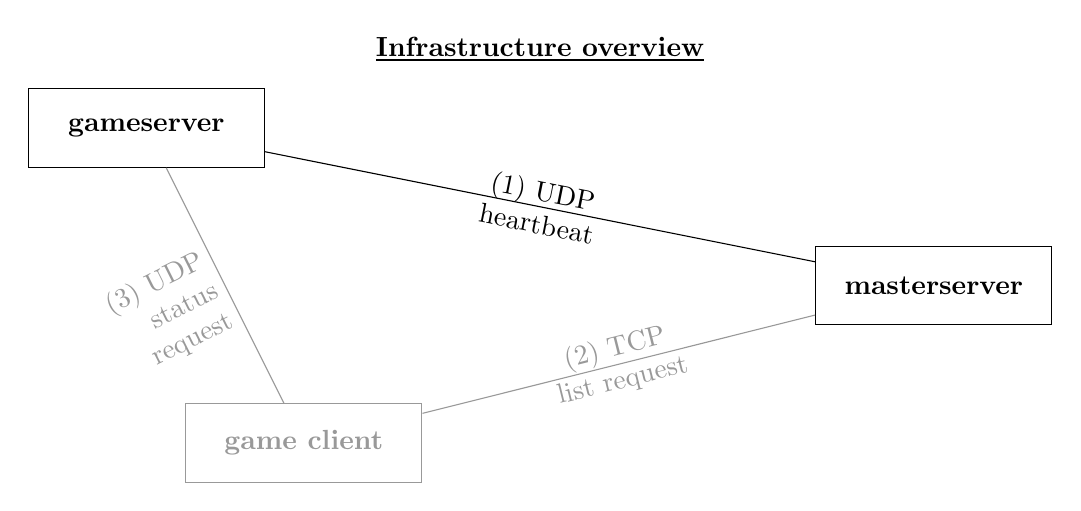
\begin{tikzpicture}

\tikzset{drawbox/.style={draw, rectangle, minimum height=1cm, minimum width=3cm}}
\tikzset{drawline/.style={midway, sloped, text width=2cm, text centered}}

% figure title
\node[rectangle] at (5, 1) (title) {\underline{\bf Infrastructure overview}};

% gameserver, masterserver, game client
\node[drawbox] at ( 0,  0) (gs) {\bf gameserver};
\node[drawbox] at (10, -2) (ms) {\bf masterserver};
\node[drawbox, black!40] at ( 2, -4) (gc) {\bf game client};

% interactions
\draw (gs) -- (ms) node[drawline] {(1) UDP\\heartbeat};
\draw[black!40] (gc) -- (ms) node[drawline] {(2) TCP\\list request};
\draw[black!40] (gc) -- (gs) node[drawline, rotate=90, left, align=right] {(3) UDP\\status request};


\end{tikzpicture}

\caption{Focus on interaction between gameserver and masterserver}\label{fig:overviewhb}
\end{figure}

\section{Exchange}
When a gameserver is first initialised, it sends a signal to the masterserver as seen in figure \ref{fig:overviewhb}. This message contains the gameservers IP-address, the port on which the hosted game is active and an acronym or shorthand name for the game title.

The masterserver receives this message or \emph{heartbeat} and processes this information. As any user or automated software can send these messages, the masterserver will attempt to authenticate the game title by challenging the gameserver with a code phrase. Both the gameserver and masterserver have the necessary algorithm to determine the expected response. The gameserver returns this response and is either rejected as an invalid sender, or acknowledged as a legitimate gameserver and added to the masterserver's list of gameservers. 

Heartbeats are sent repeatedly to indicate that a server is still active. The name ``heartbeat'' is especially similar to how we listen for heartbeats in the human body to determine if somebody is still alive. When the gameserver stops sending heartbeats, the masterserver no longer considers the gameserver active and removes it from the list.

This exchange is visualised in a diagram in figure \ref{fig:heartbeat} where the vertical axis represents passing time and the horizontal interactions correspond to the exchange discussed above.

\begin{figure}[ht]
\centering
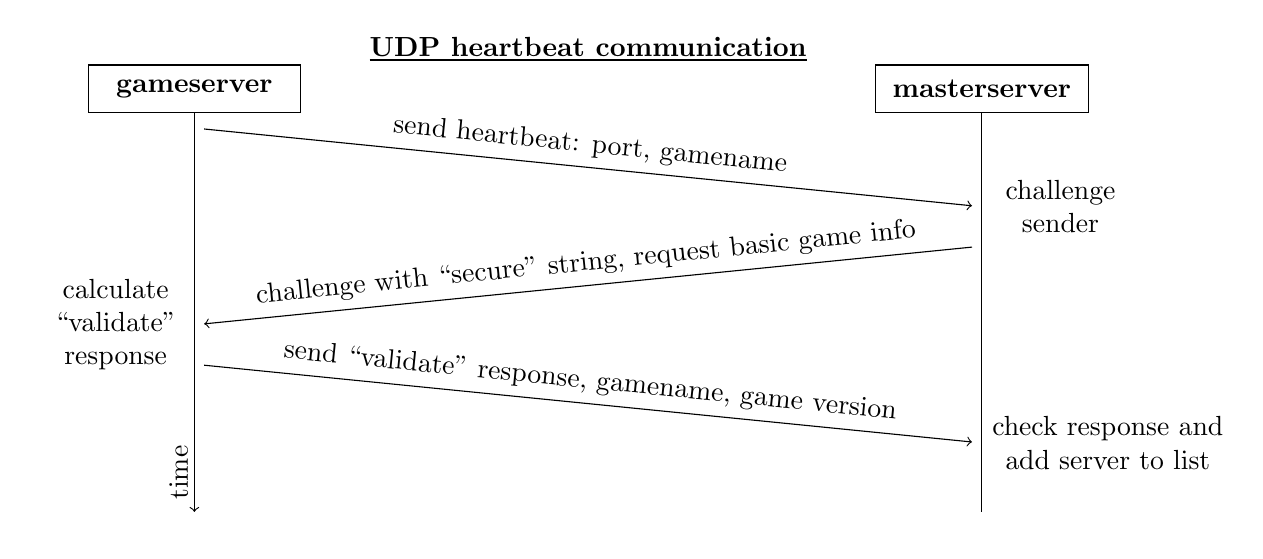
\begin{tikzpicture}

% figure title
\node[rectangle] at (5, 6) (title) {\underline{\bf UDP heartbeat communication}};

% gameserver and masterserver
\node[draw, rectangle, minimum height=0.6cm, minimum width=2.7cm] at ( 0, 5.5) (gstop) {\bf gameserver};
\node[draw, rectangle, minimum height=0.6cm, minimum width=2.7cm] at (10, 5.5) (mstop) {\bf masterserver};

% heartbeat
\node at ( 0,  5) (gshb) {};
\node at (10,  4) (mshb) {};
\node at (11,  4) (mssecure) [text width=2cm,text centered]{challenge\\sender};
\draw[->] (gshb) -- (mshb) node[midway, above, sloped] {send heartbeat: port, gamename};

% secure challenge
\node at (10,  3.5) (msse) {};
\node at ( 0,  2.5) (gsse) {};
\node at (-1,  2.5) (msvalidate) [text width=2cm,text centered]{calculate\\``validate''\\response};
\draw[->] (msse) -- (gsse) node[midway, above, sloped] {challenge with ``secure'' string, request basic game info};

% validate        
\node at ( 0,  2) (gsva) {};
\node at (10,  1) (msva) {};
\node at (11.6,  1) (mscmp) [text width=3cm, text centered]{check response and add server to list};
\draw[->] (gsva) -- (msva) node[midway, above, sloped] {send ``validate'' response, gamename,  game version};

% gameserver and masterserver bottom, vertical lines
\node at ( 0, 0) (gsbot) {};
\node at (10, 0) (msbot) {};
\draw[->] (gstop.270) -- (gsbot.90) node[at end, xshift=-0.2cm, yshift=0.5cm, rotate=90] {time};
\draw (mstop.270) -- (msbot.90) {};

\end{tikzpicture}

\caption{UDP interaction between the gameserver (left) and masterserver (right) over time.}
\label{fig:heartbeat}
\end{figure}

\section{Secure challenge}
To authenticate the validity of gameserver, masterserver and client, the GameSpy protocol introduced the \emph{secure}-challenge. In the case of a heartbeat, the masterserver attempts to authenticate the gameserver by sending it a 6-character \emph{secure} word. Both the masterserver and gameserver have a 6-character \emph{cipher} that is associated with the unique game title and perform a series of mathematical operations on the combination of the secure word and cipher. The result is a unique 8-character \emph{validate} word. If the masterserver and gameserver both arrive at the same word, the gameserver validates as legitimate and is added to the list of online gameservers.

Both the secure word and cipher may consist of any uppercase or lowercase character and any number. The validate word is a calculated response and can contain any uppercase or lowercase character and any number, but also certain special characters such as (forward) slashes, underscores and dashes. Later versions of the algorithm also allow to specify an encryption type, which results in a different validate word. The algorithm to determine the validate word consists of a series of array operations and is purely mathematical\cite{lam}.

\section{Formatting of heartbeats}
Many of the games published between 1995 and 2005 follow the GameSpy protocol\cite{gs0} and communicate heartbeats over the user datagram protocol (UDP). Sending data over UDP is fast at the risk of losing packets, corrupted packets or the information arriving out of order. Heartbeats contain only little quantities of information and are sent every few minutes, which minimises the chance and effect that data does not arrive properly.

\lstinputlisting[caption={Example of the GameSpy protocol message formatting.}, stepnumber=1, label={ls:gs0heart}]{lst/gs0heartbeat.txt}

A simple heartbeat is represented on line 1 in example \ref{ls:gs0heart}: the {\tt heartbeat} key indicates that the next value is the network port through which the gameserver can be queried and the {\tt gamename} key indicates that the following value is an acronym or shorthand for the game title. An example of how the secure challenge and response would appear is seen at lines 2 and 3.

The minimum requirement for a heartbeat is an empty UDP packet. This conveys the IP-address of the gameserver. A masterserver specifically developed to support this single game title can automatically generate the default network port and game title. However, this means that the gameserver can not be serviced on another network port and that the masterserver is limited to serving a client list \emph{only} for this specific game title. 

In order to support different network ports, a heartbeat must contain a network port (as seen in example \ref{ls:gs0heart}, line 2). A masterserver that supports multiple game titles also requires an additional key {\tt gamename}. The gamename is, as mentioned before, a unique identifier for the game title and allows the masterserver to identify which game is being serviced and authenticated\footnote{The game title and \emph{gamename} both refer to the original publications from game developers. As per the protocol, we use the word ``gamename'' to refer to these titles from now on. This term returns in chapter \ref{chap:serverlist} and \ref{chap:status}.}.

Additional information is often incorporated in the heartbeat as well. Some developers allow the indication of a new session through the {\tt statechanged} keyword, that could be used to indicate to the masterserver that a new session or map has been started. An overview of the protocol is added in appendix \ref{app:protref}.

\section{Practical execution}
In the past fifteen years, we have seen many different ways of formatting a heartbeat. It is worth noting that many game developers deviate from the specified protocol. Some games like \emph{Vietcong}, published by \emph{Gathering of Developers} in 2003, do not specify a gamename in their heartbeat, which does not make it possible to support the game on a masterserver for multiple gamenames. 

Another game, \emph{Jetfighter IV: Fortress America} published by \emph{TalonSoft} in 2000, was originally developed with a single masterserver in mind and thus did not follow protocol. The gameserver specifies the gamename {\tt jetfighter4} whereas the client specifies the gamename {\tt Jet Fighter IV} for the same game.

These inconsistencies and/or deviations from the original protocol introduce unexpected obstacles in the development process of a replacement masterserver.
